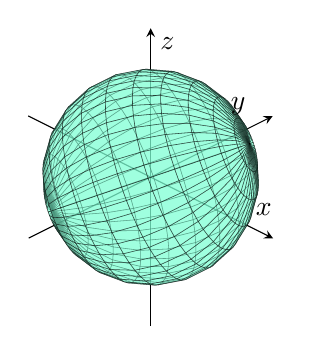
\begin{tikzpicture}
    \begin{axis}[%
        axis equal,
        width=8.5cm,
        colormap/blackwhite,
        height=8.5cm,
        axis lines = center,
        xlabel = {$x$},
        ylabel = {$y$},
        zlabel = {$z$},
        ticks=none,
        enlargelimits=0.3,
        view/h=45,
        scale uniformly strategy=units only,
    ]
    \addplot3[%
        opacity = 0.5,
        surf,
        line width=0.2pt,
        fill=Aquamarine,
        point meta=100,
        z buffer = sort,
        samples = 25,
        variable = \u,
        variable y = \v,
        domain = 0:180,
        y domain = 0:360,
    ]
    (
        {1/sqrt(2)*cos(u)*sin(v) + 0*sin(u)*sin(v) + 1/sqrt(2)*cos(v)}, % x'
        {-1/sqrt(3)*cos(u)*sin(v) - 1/sqrt(3)*sin(u)*sin(v) + 1/sqrt(3)*cos(v)}, % y'
        {-1/sqrt(6)*cos(u)*sin(v) + 2/sqrt(6)*sin(u)*sin(v) + 1/sqrt(6)*cos(v)} % z'
    );
    \end{axis}
\end{tikzpicture}